\documentclass[UTF8,a4paper,12pt]{ctexart}
\RequirePackage[left=2.6cm,right=2.6cm,top=2.7cm,bottom=2.7cm]{geometry}
\RequirePackage{amsmath,amssymb,bm}
\RequirePackage{booktabs,tabularx,multirow}
\RequirePackage{graphicx,float}
\RequirePackage{enumitem}
\RequirePackage{caption}
\RequirePackage{xcolor}
\RequirePackage{hyperref}
\RequirePackage{fancyhdr}
\RequirePackage{setspace}

% 正文只引用已经筛选确认的图片，不直接引用程序临时输出目录。
\graphicspath{{../assets/figures/selected/}}
\captionsetup{font=small,labelfont=bf,labelsep=quad,skip=6pt}
\hypersetup{
  colorlinks=true,
  linkcolor=black,
  citecolor=blue,
  urlcolor=blue
}

\setlist{nosep,leftmargin=2em}
\setlength{\parindent}{2em}
\setlength{\parskip}{0.15em}
\setlength{\headheight}{15pt}
\setlength{\emergencystretch}{2em}
\renewcommand{\arraystretch}{1.25}
\setstretch{1.22}
\setlength{\textfloatsep}{12pt plus 2pt minus 2pt}
\setlength{\floatsep}{10pt plus 2pt minus 2pt}

% 参照教师优秀进展报告：中文序号、紧凑层级、正文直接进入主题。
\ctexset{
  section={
    name={,、},
    number=\chinese{section},
    format=\heiti\zihao{-3},
    beforeskip=1.4ex plus .2ex,
    afterskip=.8ex
  },
  subsection={
    format=\heiti\zihao{4},
    beforeskip=1.2ex plus .2ex,
    afterskip=.5ex
  },
  subsubsection={
    format=\heiti\zihao{-4},
    beforeskip=1ex,
    afterskip=.4ex
  }
}

\newcommand{\ReportAuthor}{Power-Flow}
\newcommand{\ReportTitle}{潮流计算与病态收敛分析}
\newcommand{\ReportDate}{\today}

\pagestyle{fancy}
\fancyhf{}
\fancyhead[L]{\songti\zihao{5}\ReportAuthor}
\fancyhead[C]{\heiti\zihao{-4}\ReportTitle}
\fancyhead[R]{\songti\zihao{5}\ReportDate}
\fancyfoot[C]{\thepage}
\renewcommand{\headrulewidth}{0.5pt}
\renewcommand{\footrulewidth}{0pt}


\renewcommand{\ReportAuthor}{Power-Flow 项目}
\renewcommand{\ReportTitle}{潮流计算与病态收敛分析}
\renewcommand{\ReportDate}{\today}

\begin{document}

\hypersetup{pageanchor=false}
\begin{titlepage}
  \thispagestyle{empty}
  \centering
  \vspace*{2.4cm}

  {\heiti\zihao{1} 潮流计算与病态收敛分析\par}
  \vspace{0.75cm}
  {\heiti\zihao{2} 第四次汇报\par}

  \vspace{1.2cm}
  \rule{0.72\textwidth}{0.8pt}
  \vspace{1.7cm}

  \renewcommand{\arraystretch}{1.65}
  \begin{tabular}{rl}
    \heiti 项目名称： & Power-Flow 潮流计算程序\\
    \heiti 研究对象： & IEEE 3--300 节点测试系统\\
    \heiti 核心任务： & 潮流求解、算法比较与静态电压稳定分析\\
    \heiti 报告日期： & \today
  \end{tabular}

  \vfill
  \rule{0.72\textwidth}{0.4pt}
  \vspace{0.45cm}

  {\songti\zihao{-4} 基于项目概况、程序实现及实验结果编制\par}
  \vspace{1.2cm}
\end{titlepage}
\hypersetup{pageanchor=true}
\setcounter{page}{1}

\noindent 本次汇报围绕\textbf{潮流计算在正常与病态工况下的收敛问题}展开，
主要完成对潮流计算发散系统性分析。
潮流方程建模、Newton--Raphson（NR）与快速解耦法（FDLF）对比、
最优乘子法（OPF）与非线性规划法（NLP）的收敛性分析
以及连续潮流法（CPF）的稳定极限分析。
报告重点回答两个问题：
\begin{itemize}
  \item 一是”计算结果发散”究竟源于物理无解、初值吸引域还是数值过程；
  \item 二是不同算法在精度、效率和临界工况的特性。
\end{itemize}

\medskip
\noindent\textbf{本次汇报的主要结论：}
NR 在近解区域具有近二次收敛特征；
FDLF 单轮成本低，呈现线性收敛特性，但对高 $R/X$ 和临界工况更敏感；
最优乘子法与非线性规划法能够抑制发散，却可能停在非零残差点；
不同参数化方法下CPF越过鼻点的特性存在明显差异。

\section{研究背景与任务目标}
\label{sec:introduction}

潮流计算用于确定给定网络拓扑、发电计划和负荷水平下各母线电压幅值、相角及线路功率分布，
是安全校核、稳定分析和优化调度的基础。

重载、弱网、长距离辐射供电或参数尺度差异明显时，潮流方程可能无实数解，
也可能虽有解但迭代无法进入吸引域，还可能因雅可比矩阵病态而出现数值"出轨"。
因此，本任务从物理、数学和计算三个层面分析不收敛问题。

\textbf{本项目的主要任务包括：}
\begin{enumerate}
  \item 解析 IEEE 测试数据并建立母线、支路和节点导纳矩阵模型；
  \item 实现并比较牛顿--拉夫逊法与快速解耦潮流法；
  \item 开展精度、初值、负荷增长和线路参数鲁棒性测试；
  \item 测试最优乘子法与非线性规划法在临界工况下的发散与残差停滞；
  \item 测试不同参数化方法对连续潮流法跟踪 $P$--$V$ 曲线及越过鼻点能力的影响。
\end{enumerate}

\textbf{病态不收敛问题的系统认识}
通过文献调研与理论学习，本报告将不收敛区分为三个层面：
\begin{enumerate}
  \item \textbf{物理层面——解是否存在：}
  负荷增长使系统逼近静态电压稳定极限；
  在鞍结分岔点处，稳定与不稳定平衡点重合，潮流雅可比矩阵趋于奇异。
  越过极限后，原控制方式下可能不存在对应的实数平衡解。
  \item \textbf{数学层面——能否找到解：}
  NR 等局部求根算法具有有限吸引域，即使方程存在解，
  不合适的初值仍可能导致振荡、越界或收敛到其他解支。
  \item \textbf{计算层面——迭代是否稳定：}
  雅可比矩阵条件数恶化会放大舍入误差，
  过大的修正步还会使迭代偏离有效区域，
  因此需要尺度化、稳定分解和步长控制。
\end{enumerate}

\textbf{病态不收敛问题的应对方法}
针对不同的不收敛成因，有不同的处理手段：
\begin{itemize}
  \item \textbf{物理层面——逼近物理解边界：}
  连续潮流法引入延拓参数扩展潮流方程，
  使迭代在雅可比奇异时仍能沿 $P$--$V$ 曲线追踪至鞍结分岔点，
  判断该工况下解是否真实存在。
  \item \textbf{数学层面——扩大吸引域：}
  非线性规划法将潮流方程转化为残差范数最小化问题，
  通过全局寻优降低对初值质量的依赖。
  \item \textbf{计算层面——改善数值稳定性：}
  标幺化消除量级差异（尺度化），
  带主元选取的 LU 分解避免小主元除零（稳定分解），
  最优乘子法沿 NR 方向一维寻优限制修正幅度（步长控制）；
  此外，迭代顺序与数值截断策略也对稳定性有一定影响。
\end{itemize}

\section{潮流问题建模}
\label{sec:model}

设节点导纳矩阵为 $\bm{Y}=\bm{G}+\mathrm{j}\bm{B}$，节点 $i$ 的电压为 $V_i\angle\theta_i$，则节点注入功率为
\begin{align}
P_i(\bm{x})&=V_i\sum_{j=1}^{n}V_j
\left[G_{ij}\cos(\theta_i-\theta_j)+B_{ij}\sin(\theta_i-\theta_j)\right],\\
Q_i(\bm{x})&=V_i\sum_{j=1}^{n}V_j
\left[G_{ij}\sin(\theta_i-\theta_j)-B_{ij}\cos(\theta_i-\theta_j)\right].
\end{align}

根据平衡、PV 和 PQ 节点的已知量，潮流方程可统一表示为
\begin{equation}
\bm{f}(\bm{x})=
\begin{bmatrix}
\bm{P}^{\mathrm{spec}}-\bm{P}(\bm{x})\\
\bm{Q}^{\mathrm{spec}}-\bm{Q}(\bm{x})
\end{bmatrix}=\bm{0}.
\label{eq:power-flow}
\end{equation}

对基准负荷引入统一增长参数 $\lambda$：
\begin{equation}
P_{L,i}(\lambda)=(1+\lambda)P_{L,i}^{0},\qquad
Q_{L,i}(\lambda)=(1+\lambda)Q_{L,i}^{0}.
\end{equation}
由此得到 $\bm{f}(\bm{x},\lambda)=\bm{0}$。随着负荷增长，解沿高电压分支向鼻点移动；鼻点处雅可比矩阵趋于奇异，对应静态电压稳定极限。


\section{潮流求解方法}
\label{sec:methods}

\subsection{牛顿--拉夫逊法}

牛顿--拉夫逊法是潮流方程的经典求解方法\cite{tinney1967}，在每轮迭代中求解
\begin{equation}
\bm{J}(\bm{x}^{(k)})\Delta\bm{x}^{(k)}=-\bm{f}(\bm{x}^{(k)}),\qquad
\bm{x}^{(k+1)}=\bm{x}^{(k)}+\Delta\bm{x}^{(k)}.
\end{equation}
当初值接近非奇异解时，该方法通常具有二次收敛特征，但每轮需要重新构造并分解雅可比矩阵。

\subsection{快速解耦潮流法}

快速解耦法利用 $P$--$\theta$ 与 $Q$--$V$ 的主导耦合关系\cite{stott1974}，将迭代近似分解为
\begin{equation}
\bm{B}'\Delta\bm{\theta}=\Delta\bm{P}/\bm{V},\qquad
\bm{B}''\Delta\bm{V}=\Delta\bm{Q}/\bm{V}.
\end{equation}
固定系数矩阵可以预先分解，因此单轮成本低；但高 $R/X$、强耦合或临界工况会削弱其近似条件。

\subsection{全局化方法与连续潮流}

最优乘子法在牛顿方向上搜索合适步长，非线性规划法最小化 $\tfrac12\|\bm{f}(\bm{x})\|_2^2$。它们可以抑制迭代发散，但也可能停在非零残差的最小二乘点。

连续潮流法采用预测--校正策略跟踪 $\bm{f}(\bm{x},\lambda)=\bm{0}$ 的解流形\cite{ajjarapu1992}，并在鼻点附近使用局部或伪弧长等参数化绕开自然参数化的奇异。项目当前支持自然、伪弧长、切线角和绝对 $V/P$ 角参数化。

\subsection{方法之间的定位关系}

NR 与 FDLF 用于求取给定参数下的离散运行点；最优乘子和非线性规划用于改善定点求解过程的全局性；CPF 则用于追踪随负荷参数连续变化的解分支。前三类方法回答“当前运行点能否求出”，CPF 回答“运行点如何随参数演化并在何处达到极限”。因此，算法比较不能只比较耗时，还应同时报告最终残差、步长控制量、无功限值状态和所处解支。

\section{程序实现与试验设计}
\label{sec:experiments}

程序采用分层结构：
\texttt{core} 负责电网对象、导纳矩阵和功率方程；
\texttt{solvers} 提供统一求解接口；
\texttt{cpf} 负责专门对连续潮流进行预测、校正、参数化和步长控制；
\texttt{analysis} 比较分析算法、鲁棒性、临界停滞与规模增长。

为保证结果可比较，所有算法使用相同的输入数据、初值规则和残差定义；
重复计时先执行一次预热，再按单侧 Tukey--IQR 规则识别异常耗时。
临界负荷测试开启发电机无功限值及 PV--PQ 转换，
并分别记录“方程残差满足阈值”和“算法停止但残差非零”两类状态。

\begin{table}[H]
\centering
\caption{主要试验设置}
\label{tab:settings}
\begin{tabularx}{\textwidth}{p{3.8cm}X}
\toprule
项目 & 设置\\
\midrule
测试系统 & IEEE 3、4、5、9、14、30、39、43、57、118、145、162 和 300 节点\\
基础条件 & 100 MVA；平坦启动；基础收敛精度 $10^{-6}$\\
重复计时 & 每种算法运行 11 次，第 1 次预热，正式样本采用单侧 IQR 规则识别异常值\\
精度扫描 & $10^{-4}$、$10^{-6}$、$10^{-8}$、$10^{-10}$\\
初值扰动 & 电压幅值 $\pm2\%$、$\pm5\%$、$\pm10\%$；相角 $\pm2^\circ$、$\pm5^\circ$、$\pm10^\circ$\\
病态工况 & 负荷倍率 1.600--1.620；线路电阻倍率 1、2、3；开启 PV--PQ 转换\\
\bottomrule
\end{tabularx}
\end{table}

\section{结果与分析}
\label{sec:results}

\subsection{全算例收敛与效率}

现有结果表明，NR 在多数算例中用较少迭代完成求解，观测收敛阶接近 2；FDLF 的迭代次数更多、观测阶接近 1，但其固定矩阵可以重复利用，总耗时通常更低。

\begin{figure}[p]
\centering
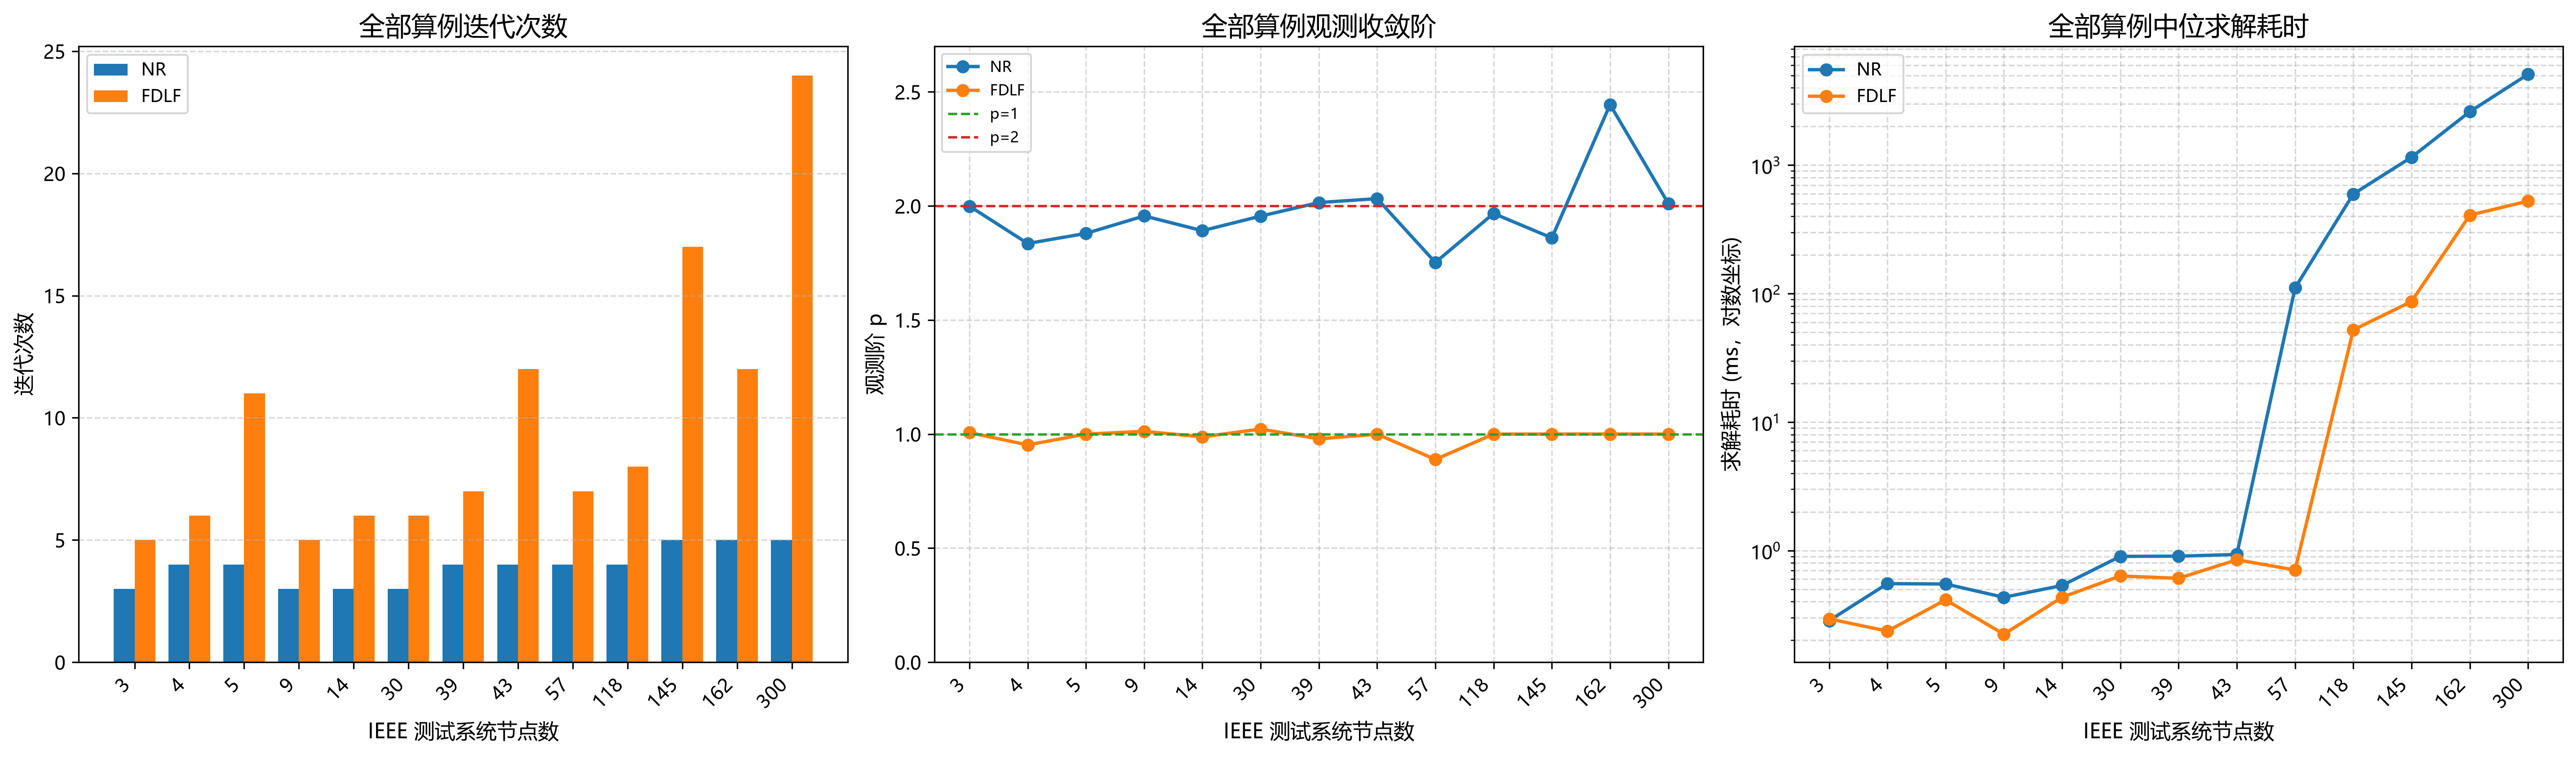
\includegraphics[width=\textwidth]{Solver_All_Cases_Summary.png}
\caption{IEEE 全部算例的迭代次数、收敛阶和中位求解耗时}
\label{fig:all-cases}
\end{figure}

从图~\ref{fig:all-cases}可以得到两点认识：其一，迭代次数不能直接代表总耗时，FDLF 通过复用系数矩阵以更多迭代换取更低单轮成本；其二，规模增大后两种算法的耗时均明显上升，线性方程组求解逐渐成为主要瓶颈。

\subsection{IEEE 118 节点详细比较}

在 $10^{-6}$ 精度和平坦启动条件下，118 节点算例中 NR 与 FDLF 分别约用 4 轮和 8 轮。现有结果中的 NR 中位耗时为 71.400 ms，FDLF 中位耗时为 6.983 ms，后者约快 10.2 倍。该倍数仅代表当前代码、配置与运行环境。

\begin{figure}[p]
\centering
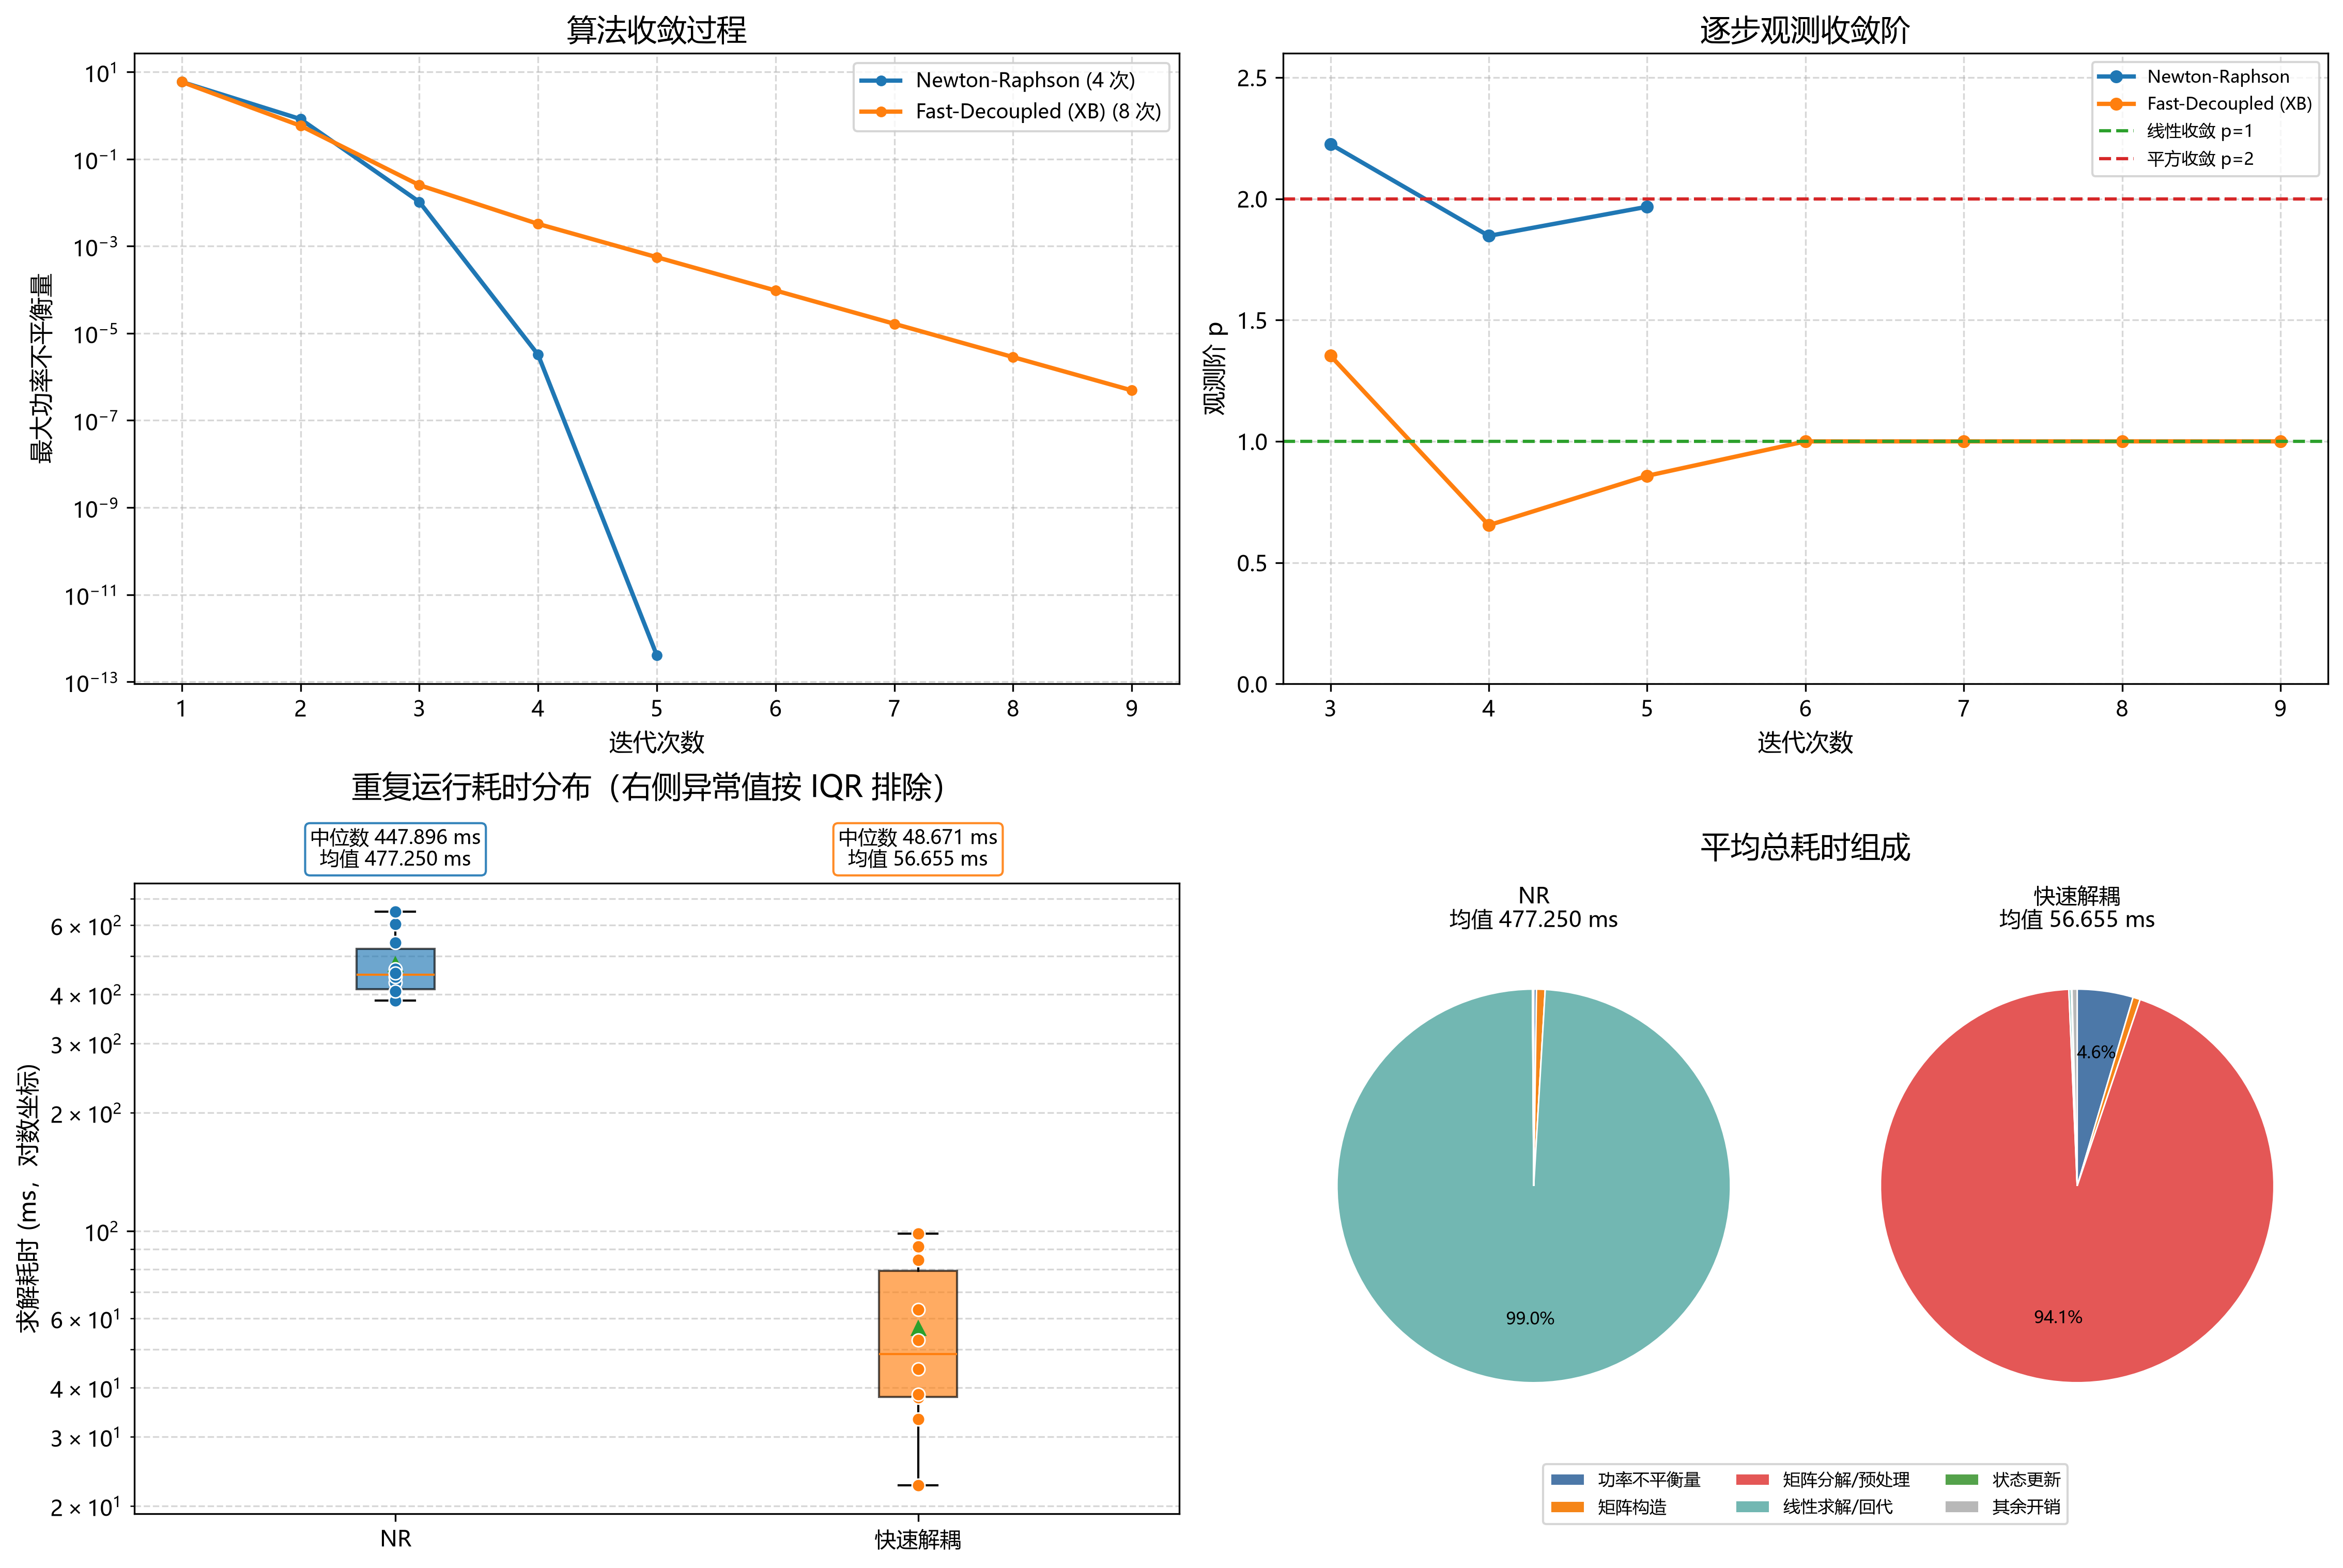
\includegraphics[width=\textwidth]{Solver_118_NR_FDLF_Comparison.png}
\caption{IEEE 118 节点系统 NR 与 FDLF 的收敛和耗时分解}
\label{fig:118-comparison}
\end{figure}

图~\ref{fig:118-comparison}进一步说明，NR 的主要开销集中在线性求解与回代，FDLF 的主要开销集中在固定矩阵的预处理。NR 的残差在后期快速下降，体现局部二次收敛；FDLF 则保持近线性下降。二者最终状态的一致性应通过母线电压、相角和功率残差共同校核。

\subsection{鲁棒性与临界状态}

常规初值扰动下两种算法均保持较高成功率。负荷逼近临界区域或线路 $R/X$ 增大后，FDLF 的迭代次数与失败概率增长更明显。最优乘子和非线性规划虽然能抑制发散，但若最终残差高于阈值，只能判定为残差停滞，不能视为潮流收敛。

\begin{figure}[p]
\centering
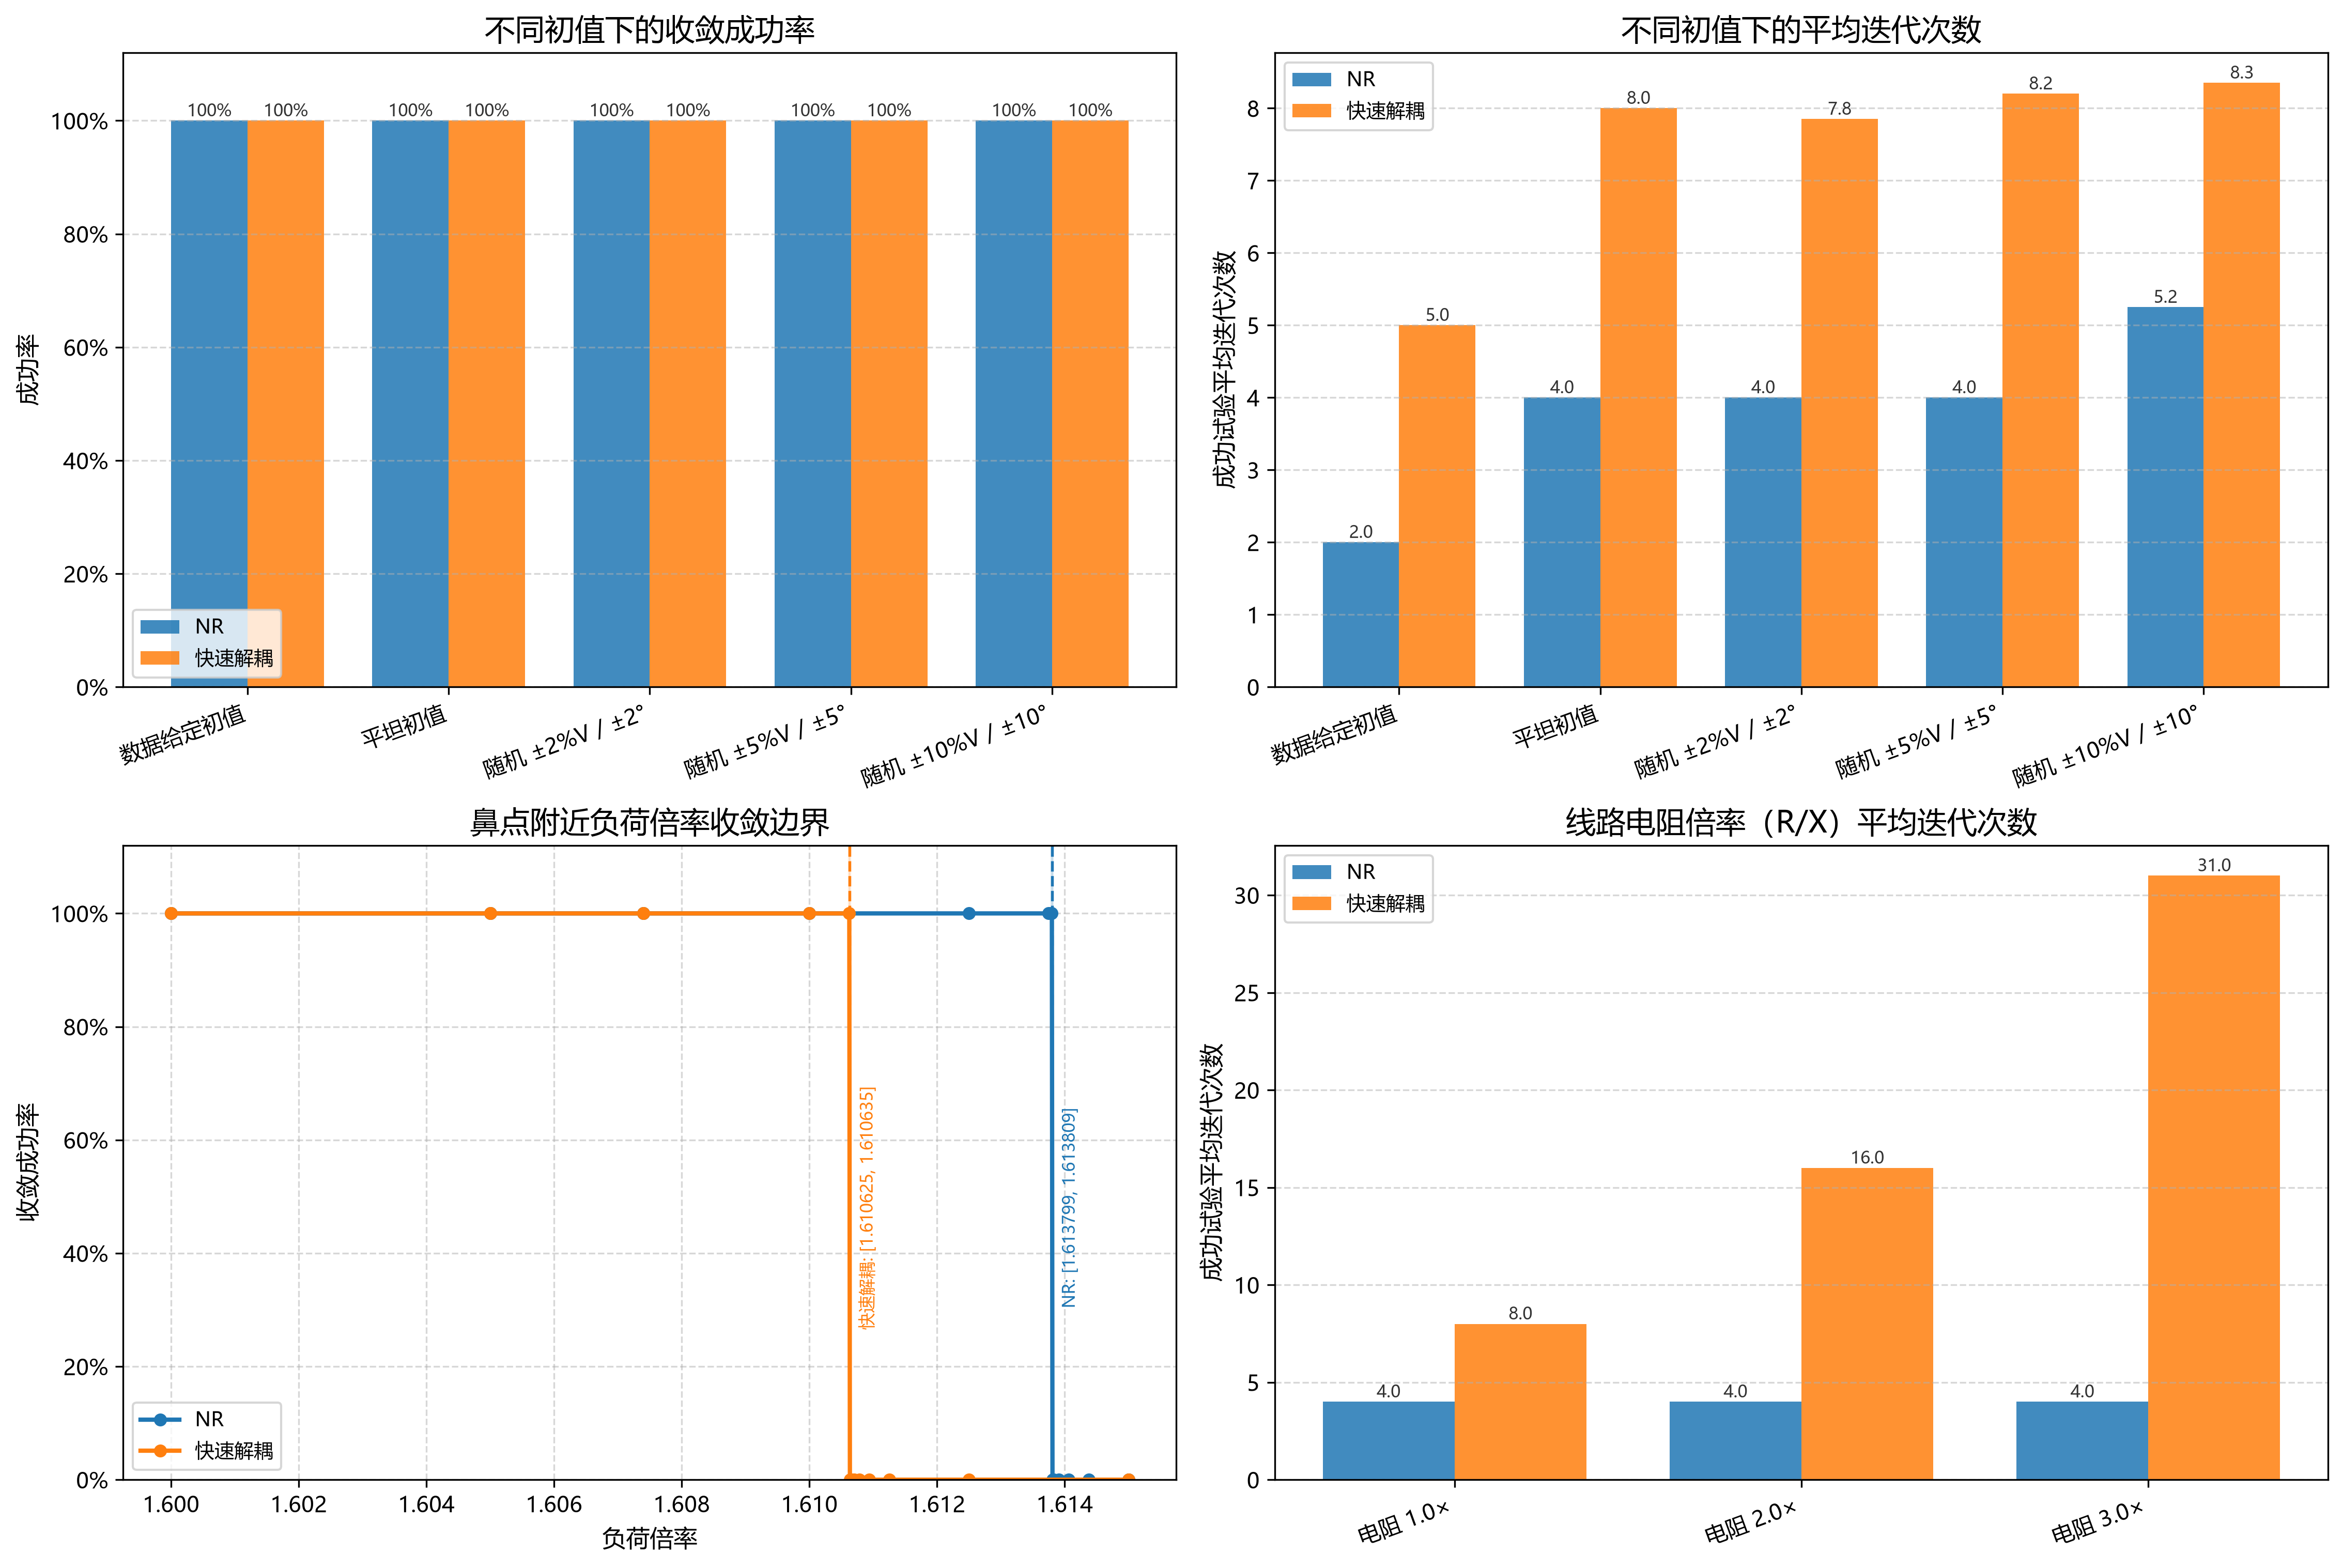
\includegraphics[width=\textwidth]{Solver_118_Robustness.png}
\caption{IEEE 118 节点系统的初值、负荷与线路参数鲁棒性}
\label{fig:robustness}
\end{figure}

\begin{figure}[p]
\centering
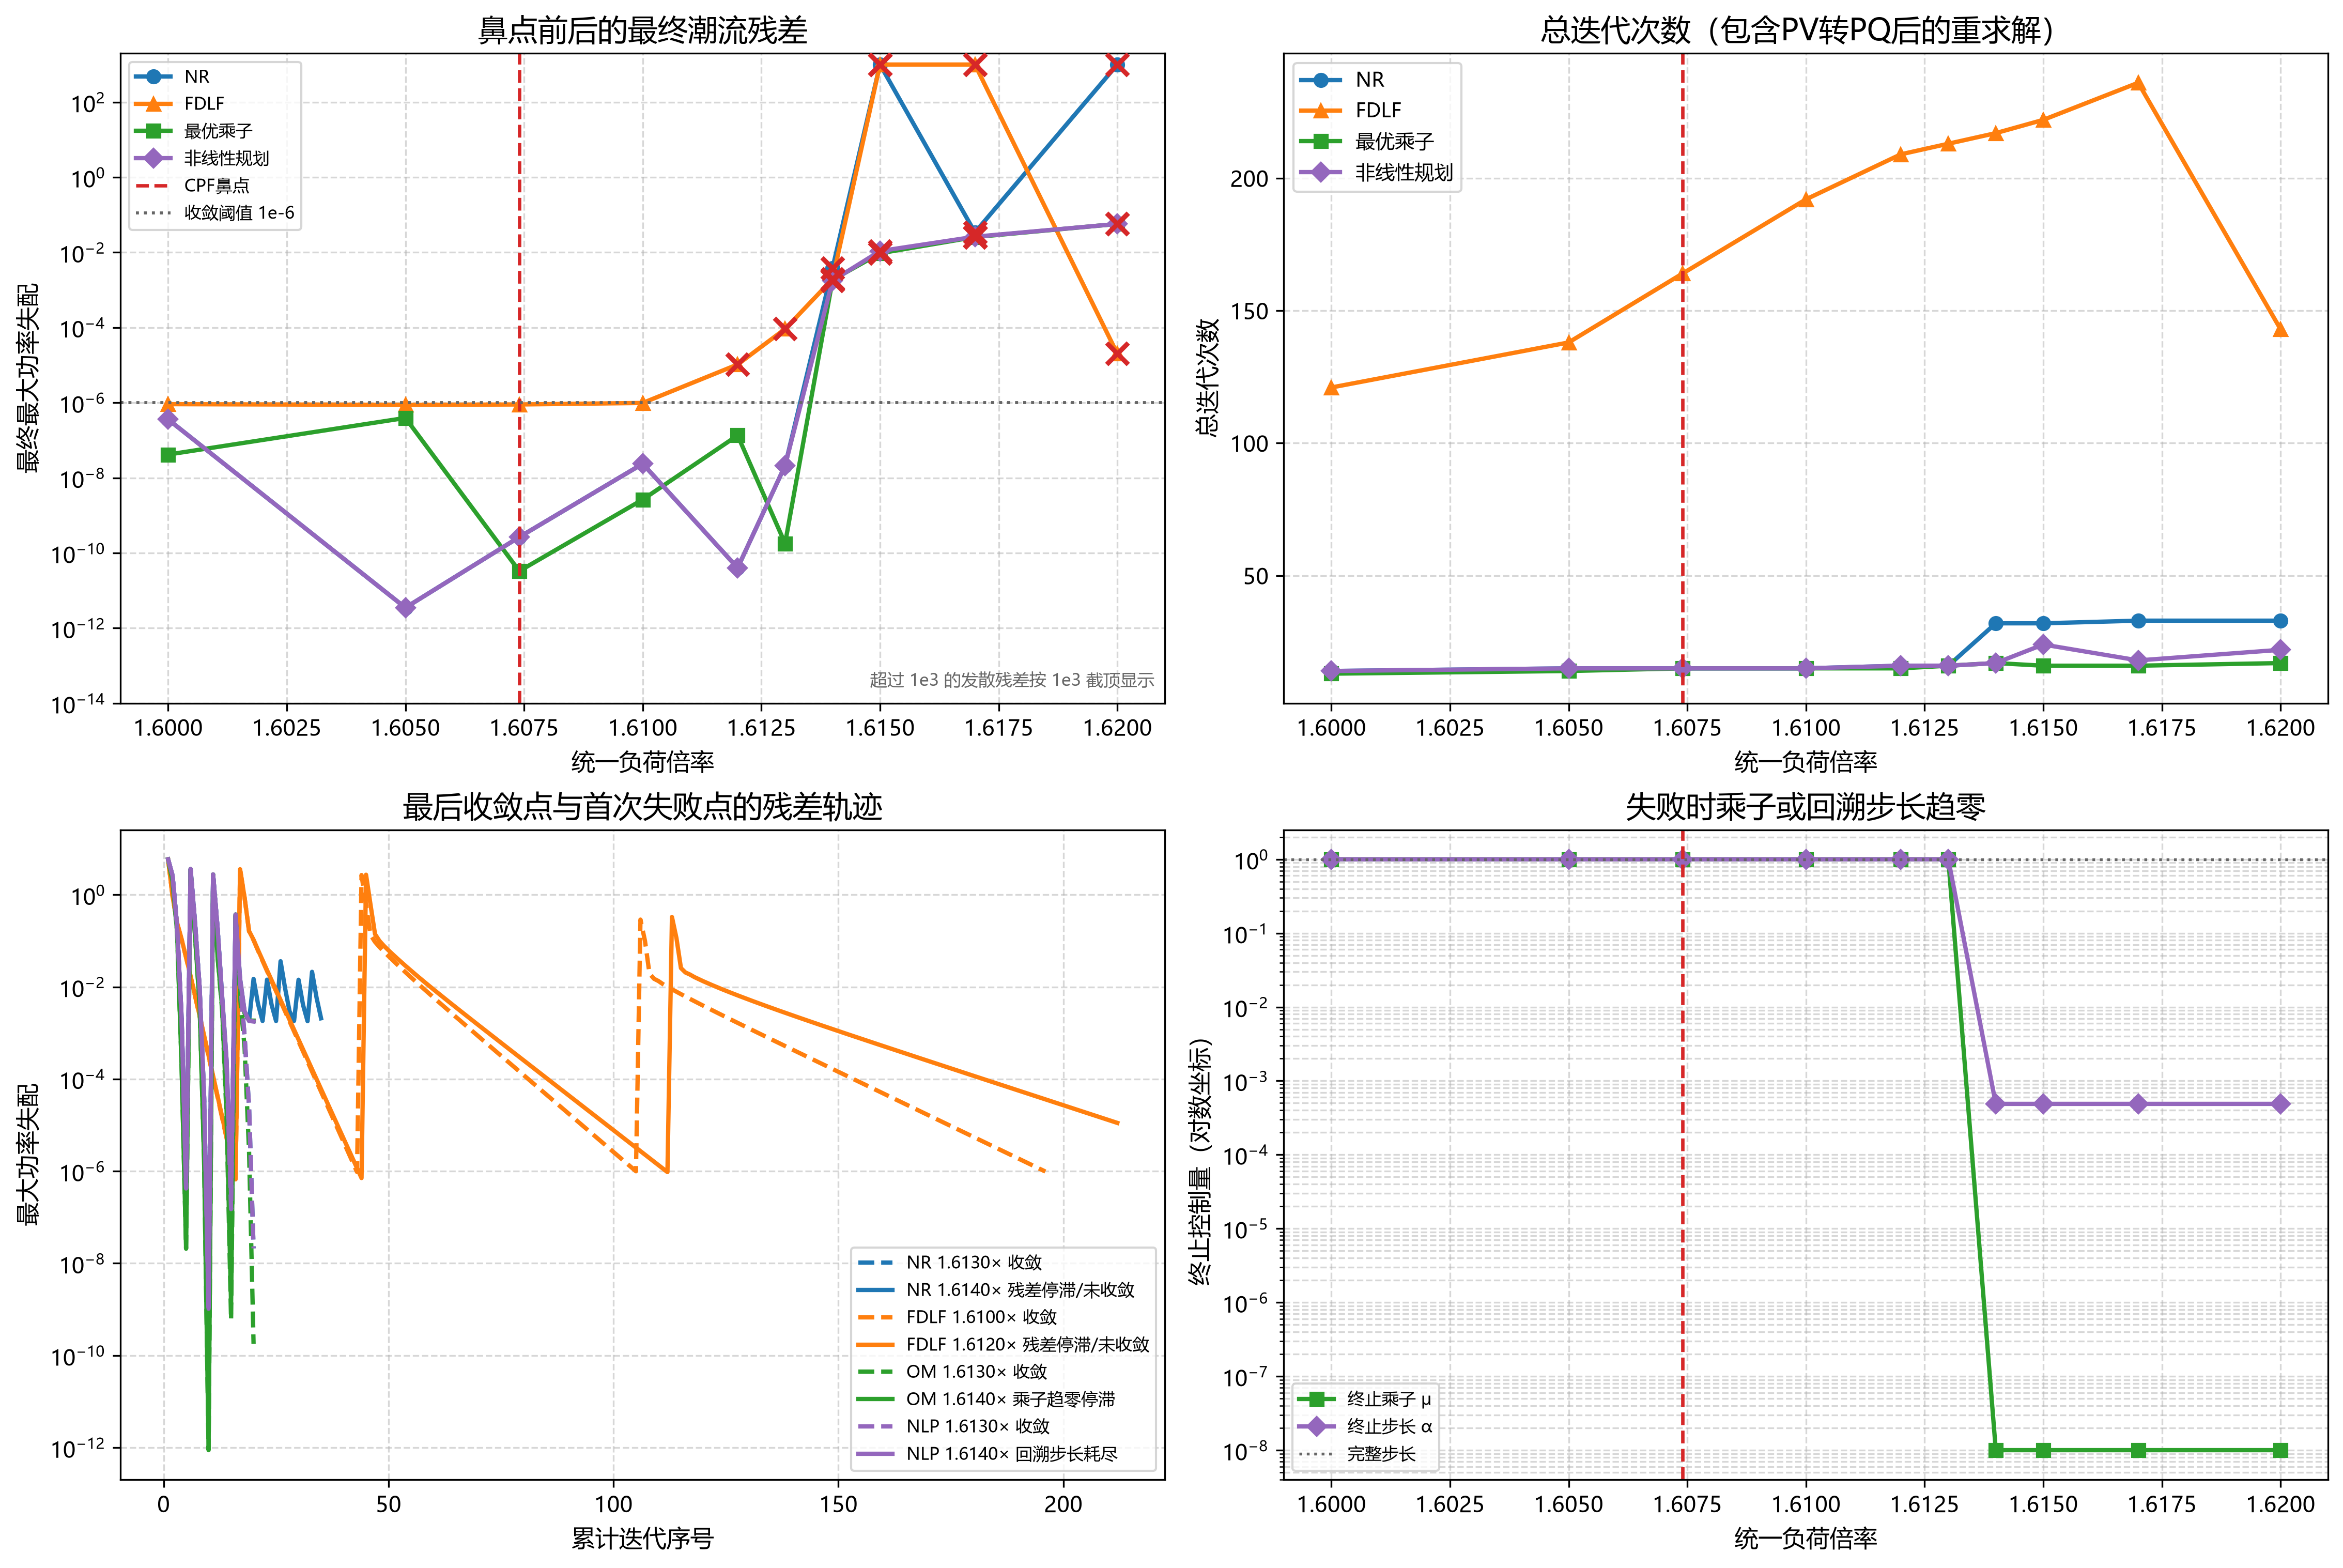
\includegraphics[width=\textwidth]{Solver_118_Critical_Stagnation.png}
\caption{IEEE 118 节点系统在参考鼻点前后的残差与控制量}
\label{fig:critical}
\end{figure}

这里需要特别区分\textbf{物理稳定极限}与\textbf{数值收敛边界}。CPF 参考鼻点来自连续解分支；NR 或 FDLF 的最后收敛倍率则依赖初值、容差、迭代上限和 PV--PQ 转换规则。两者定义不同，若固定点算法在参考鼻点后仍返回结果，应优先核查方程集合、最终残差和解支，而不能直接提高系统稳定极限。

\subsection{规模增长特征}

当前结果显示，系统规模增大后矩阵构造与分解成本迅速增长。后续采用稀疏矩阵装配、稀疏分解和符号分解复用具有明确价值。

\begin{figure}[p]
\centering
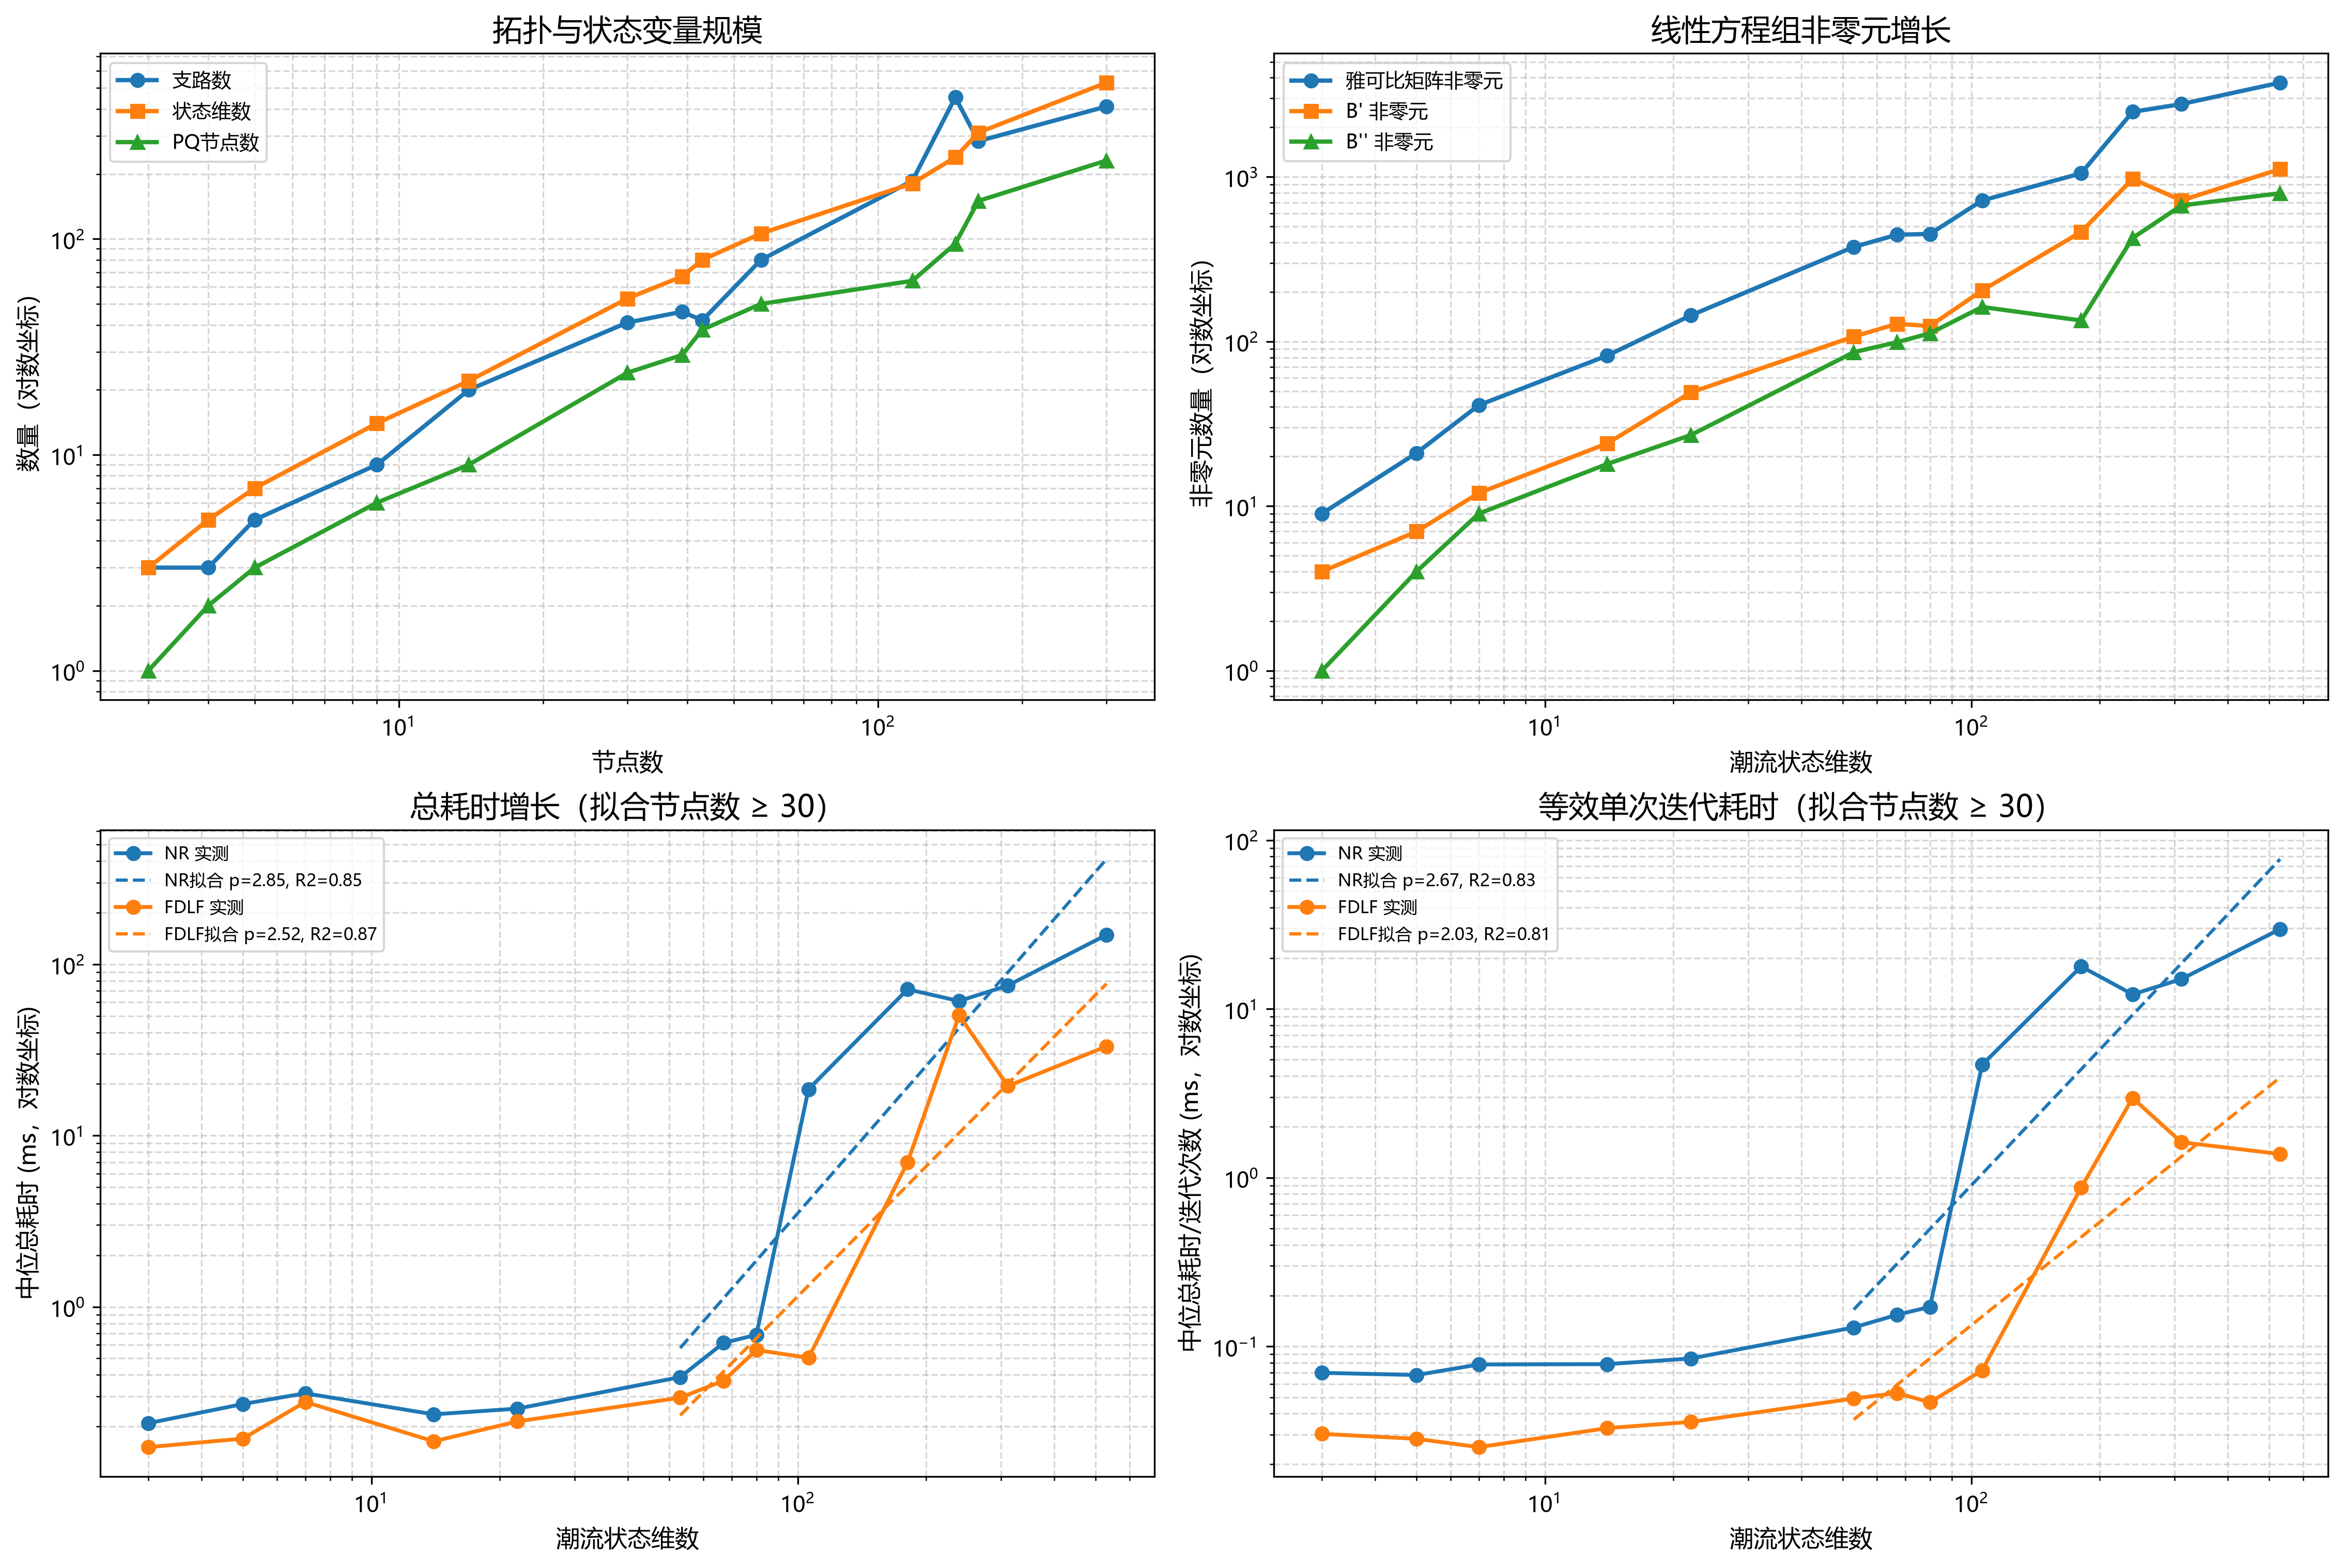
\includegraphics[width=\textwidth]{Solver_Scaling_Trend.png}
\caption{网络拓扑、矩阵非零元及求解耗时的规模增长趋势}
\label{fig:scaling}
\end{figure}

以节点数不少于 30 的算例拟合，当前实现中 NR 总耗时和单轮耗时对状态维数的增长指数分别约为 2.85 和 2.67，FDLF 分别约为 2.52 和 2.03。该结果说明当前实现仍带有明显的稠密线性代数特征，稀疏化是比微调迭代公式更优先的工程改进方向。

\clearpage

\section{文献阅读}
\label{sec:literature-review}

除程序实现和算例分析外，本项目还围绕潮流计算、病态机理与静态电压稳定阅读了相关
书籍和论文。以下简要介绍对本文影响较大的内容。

\subsection{《高等电力网络分析》（张伯明、严正）}

该书帮助我系统梳理了潮流计算的数学模型、基本算法及发展过程，并补充了特殊潮流、
随机潮流和潮流跟踪等扩展内容。其中，连续潮流法的详细介绍打下基础。

另一个很有趣的内容是快速解耦法中的迭代取用顺序将内涵标准NR法迭代的主要耦合影响因素，
为快速解耦法的广泛适用范围做出解释。

\subsection{《雅可比矩阵对直角坐标牛顿法潮流计算收敛性影响的研究》}

该文的背景介绍部分对病态潮流的发展和相关研究进行了较完整的梳理，
提供了零散的病态原因以及病态算法，
本文进一步归纳出病态成因的物理可解性、初值吸引域和数值迭代过程的三级分类。

\subsection{《基于张量法的电力系统病态潮流求解与 \(P\)--\(V\) 曲线》}

该文介绍了不同于 NR 和快速解耦法的张量潮流方法。其对非线性模型和迭代格式的扩展
幅度大于最优乘子法，为理解病态潮流中改善收敛性的其他技术路线提供了对照。

\subsection{《基于连续潮流的电力系统电压稳定性研究》}

该文与《高等电力网络分析》共同加深了本文对标准连续潮流流程的认识，并重点启发了
对自然、弧长和绝对角度等不同参数化方式的比较，本文进一步适用了切线角度进行了尝试分析。

\subsection{《电力系统潮流的病态性及其算法研究》}

该文从同伦方法的角度解释了连续潮流的数学基础，使本文认识到 CPF 可以看作同伦思想
在潮流计算中的一种具体形式；通过调整同伦函数和延拓参数，还可以进一步改善复杂工况
下的跟踪与收敛性能。

\section{总结与下一步工作}
\label{sec:conclusion}

本任务已经形成从数据解析、基础潮流到临界稳定分析的工作流。
NR 具有近解区域的快速收敛能力，FDLF 具有较低的单轮计算成本，但对高 $R/X$ 和强耦合工况更敏感。
接近稳定极限后，算法应当结合最终残差、无功限值、雅可比奇异性和连续潮流分支综合判断。

\subsection{当前结论}

\begin{enumerate}
  \item 常规工况下 NR 与 FDLF 均能可靠求解，前者迭代少，后者单轮成本低；
  \item 全局化方法在本0~300的小规模系统中对于负荷统一增长的病态收敛优化不明显；
  \item 各种参数化的 CPF 各有优劣。与奇异性指标及矩阵条件数可作为最大负荷能力判断的依据。
\end{enumerate}

\subsection{当前不足}

目前 CPF 结果有待进一步整理分析，对于错误分支的产生与特点认识不足。
规模分析也仍基于当前 Python 与矩阵实现，尚未区分算法复杂度。

\subsection{下一步工作}

后续工作建议如下：
\begin{enumerate}
  \item 统一不同求解器的负荷参数化、PV--PQ 转换与残差口径；
  \item 增加雅可比最小奇异值、条件数和临界特征向量监测；
  \item 引入稀疏矩阵存储与稀疏 LU/QR 分解；
  \item 在故障、非均匀负荷增长等场景下复核 CPF 参数化选择，并区分纯参数化与后备接管的贡献；
  \item 保存配置、代码版本、原始数据和图像来源，提高结果可复现性。
\end{enumerate}


\subsection{探索性内容}

按照《高等电力网络分析 (张伯明，严正著)》中的证明
及《PQ分解法解潮流方程收敛性的影响因素分析_王若涵》中关于迭代顺序的研究进行讨论验证。

\clearpage
\nocite{*}
\bibliographystyle{plain}
\bibliography{../references/references}

\end{document}
